\section{Allgemeine Funktionsweise (AW)}
Der Kunde eines Fotografen bekommt nach einer Fotositzung (Session) eine Karte mit 
einer Session-ID überreicht. Anhand dieser ID, welche sich in der aufgerufenen 
Anwendung eingeben lässt, werden die Bilder aus der Session beim Kunden im Endgerät
(Desktop-Browser oder Smartphone-Browser) dargestellt.

Der generelle Aufbau lässt sich der folgenden Abbildung \ref{fig_genereller_aufbau} entnehmen.

\begin{figure}[h]
	\centering
	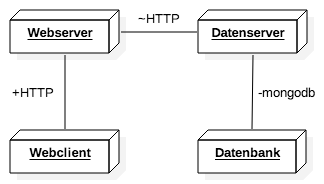
\includegraphics[width=14cm]{bilder/genereller_aufbau}
	\caption{Genereller Aufbau der Anwendung}
	\label{fig_genereller_aufbau}
\end{figure}

Wie in der Grafik zu sehen ist, besteht die Anwendung aus vier den Komponenten
\begin{itemize}
	\item \textbf{Webclient}: diese Komponente ist für den Nutzer sichtbar und dient der Interaktion mit der Anwendung
	\item \textbf{Webserver}: der Webserver nimmt Anfragen des Clients entgegen, beantwortet sie entweder selber oder leitet sie an den Datenserver weiter und gibt Antworten des Datenservers an den Webclient weiter
	\item \textbf{Datenserver}: der Datenserver nimmt Anfragen des Webservers entgegen und dient der Interaktion mit der Datenbank
	\item \textbf{Datenbank}: die Datenbank dient der persistenten Haltung von Sitzungsdaten und Fotos
\end{itemize}

Im Folgenden werden die einzelnen Komponenten weiter vorgestellt und ihre Funktionsweise erläutert.